\documentclass[conference]{IEEEtran}
\usepackage{amsmath,amssymb}
\usepackage{booktabs}
\usepackage{graphicx}
\graphicspath{{figures/}{./}{reports/figures/}}
\usepackage{xcolor}
\usepackage{cite}
\usepackage{url}
% Marks text you must replace with your own results or wording before submission.
\newcommand{\TODO}[1]{\textcolor{red}{[#1]}}

\begin{document}

\title{Remaining Useful Life Prediction for Industrial Engines:\\
A Feature-Engineering Machine Learning Baseline on NASA C-MAPSS}

\author{\IEEEauthorblockN{\TODO{Member 1}, \TODO{Member 2}, \TODO{Member 3}, \TODO{Member 4}, \TODO{Member 5}}
\IEEEauthorblockA{\TODO{Department, Institution}\\
\TODO{emails}}}

\maketitle

\begin{abstract}
Predictive maintenance requires estimating how many operating cycles an engine has left before failure, its Remaining Useful Life (RUL). We study this regression problem on the NASA C-MAPSS FD001 turbofan dataset. We build a machine learning baseline from engineered degradation features: rolling means, rolling slopes, and a health measure that tracks drift from each engine's own healthy start. We compare a naive mean baseline, an Elastic Net, and a Random Forest using 5-fold cross-validation grouped by engine, and then evaluate once on the held-out test engines. The Random Forest reaches a cross-validated RMSE of 34.78 and MAE of 22.79 cycles (naive baseline: 68.87 and 56.86; Elastic Net: 40.04 and 30.63) and a test RMSE of 23.34 and MAE of 15.58 cycles on the 100 test engines. Errors are far smaller near failure (test MAE 4.02 for true RUL below 50) than early in life (20.54). We discuss the limits of fixed-window features, which motivate sequence models in the next phase of this work.
\end{abstract}

\begin{IEEEkeywords}
remaining useful life, predictive maintenance, C-MAPSS, feature engineering, random forest, elastic net
\end{IEEEkeywords}

\section{Introduction}
Engines degrade gradually, and their sensor readings drift as components wear. Estimating RUL lets operators schedule maintenance before a failure without replacing parts too early. The task is a regression problem: given the sensor history of an engine up to a cycle $t$, predict the number of cycles remaining.

This report covers the first phase of the project, a classical machine learning baseline. Its goals are (i) to build interpretable degradation features, (ii) to compare simple and flexible regressors under a leakage-free, engine-level evaluation, and (iii) to identify where fixed-window features fall short. Contributions:
\begin{itemize}
\item A causal feature set built from per-engine rolling statistics and a drift-from-healthy measure.
\item An evaluation grouped by engine, with a naive baseline, a linear model, and a tree ensemble.
\item An error analysis by degradation stage and a controlled comparison of capped versus uncapped training targets.
\end{itemize}

\section{Related Work}
\TODO{Rewrite this section in your own words after reading each paper, and add one or two further RUL papers you found yourselves. Verify every citation.}
Saxena et al.\ \cite{saxena2008damage} describe the damage propagation model behind the C-MAPSS simulations, and the dataset is distributed through the NASA Prognostics Data Repository \cite{saxena2008cmapss}. Recurrent and convolutional networks have been applied to RUL estimation on this benchmark \cite{heimes2008rnn,babu2016cnn}, and the LSTM \cite{hochreiter1997lstm} is a common choice for sequences. On the classical side, Random Forests \cite{breiman2001rf} and regularised linear models such as the Elastic Net \cite{zou2005en} are standard tabular baselines, and we use their scikit-learn implementations \cite{pedregosa2011sklearn}.

\section{Dataset and Exploratory Analysis}
\subsection{C-MAPSS FD001}
The FD001 subset contains 100 training engines run to failure and 100 test engines that stop before failure. Each row is one engine at one cycle with three operating settings and 21 sensor readings. FD001 has a single operating condition and a single fault mode. The training set has 20{,}631 rows and the test set 13{,}096 rows. The true RUL at the last cycle of each test engine is provided separately.

\subsection{Data quality}
We checked for missing values, duplicate rows, duplicate (engine, cycle) pairs, data types, and cycle continuity. No missing values or duplicate rows were found in the training, test, or RUL files, there were no duplicate (engine, cycle) pairs, and every engine in both sets starts at cycle 1 with consecutive cycles.

\subsection{Exploratory findings}
Engine lifetimes range from 128 to 362 cycles (mean 206.3, median 199, std 46.3), so about 38.9\% of training rows have RUL above 125 (Fig.~\ref{fig:eda}). Several sensors drift toward failure (s2, s3, s4 and s11 rise; s7 and s12 fall), staying close to flat early in life and changing faster over roughly the last 150 to 200 cycles, with substantial noise (Fig.~\ref{fig:sensors}). Sensors s1, s5, s10, s16, s18 and s19 are constant, and s6 takes only two values. Spearman correlation with RUL is strongest for the cycle number ($-0.79$) and for s11, s4, s12, s7 and s15 (absolute value $0.67$ to $0.72$). Operating setting op3 is constant, and op1 and op2 vary only in the third and fourth decimal, so FD001 behaves as a single operating condition.
Engine lifetimes vary widely, so training rows are concentrated at high RUL, and only a minority lie in the last 50 cycles. Some sensors drift toward failure while others are essentially constant. The operating settings vary only by small amounts in FD001, so they describe noise rather than regime changes and are not used as features.

\begin{figure}[t]
\centering
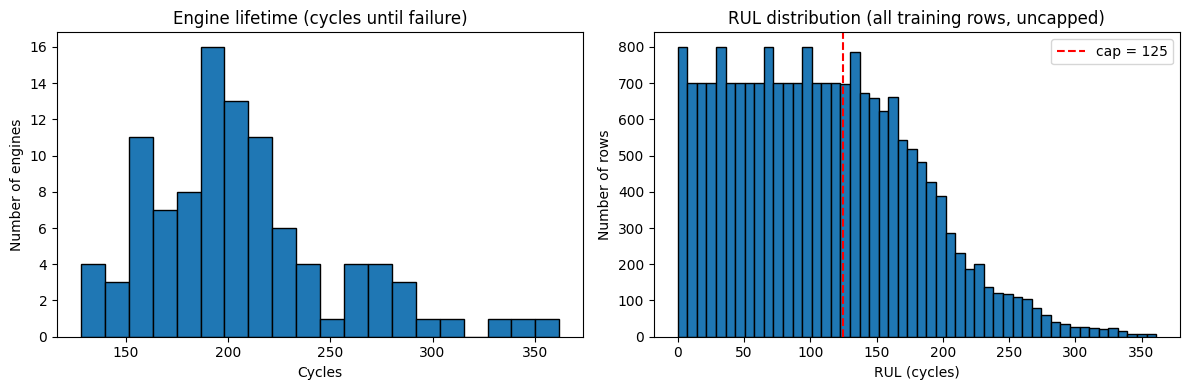
\includegraphics[width=\columnwidth]{figures/lifetime_rul.png}
\caption{Engine lifetimes (left) and RUL distribution of training rows (right); the dashed line marks 125 cycles.}
\label{fig:eda}
\end{figure}

\begin{figure*}[t]
\centering
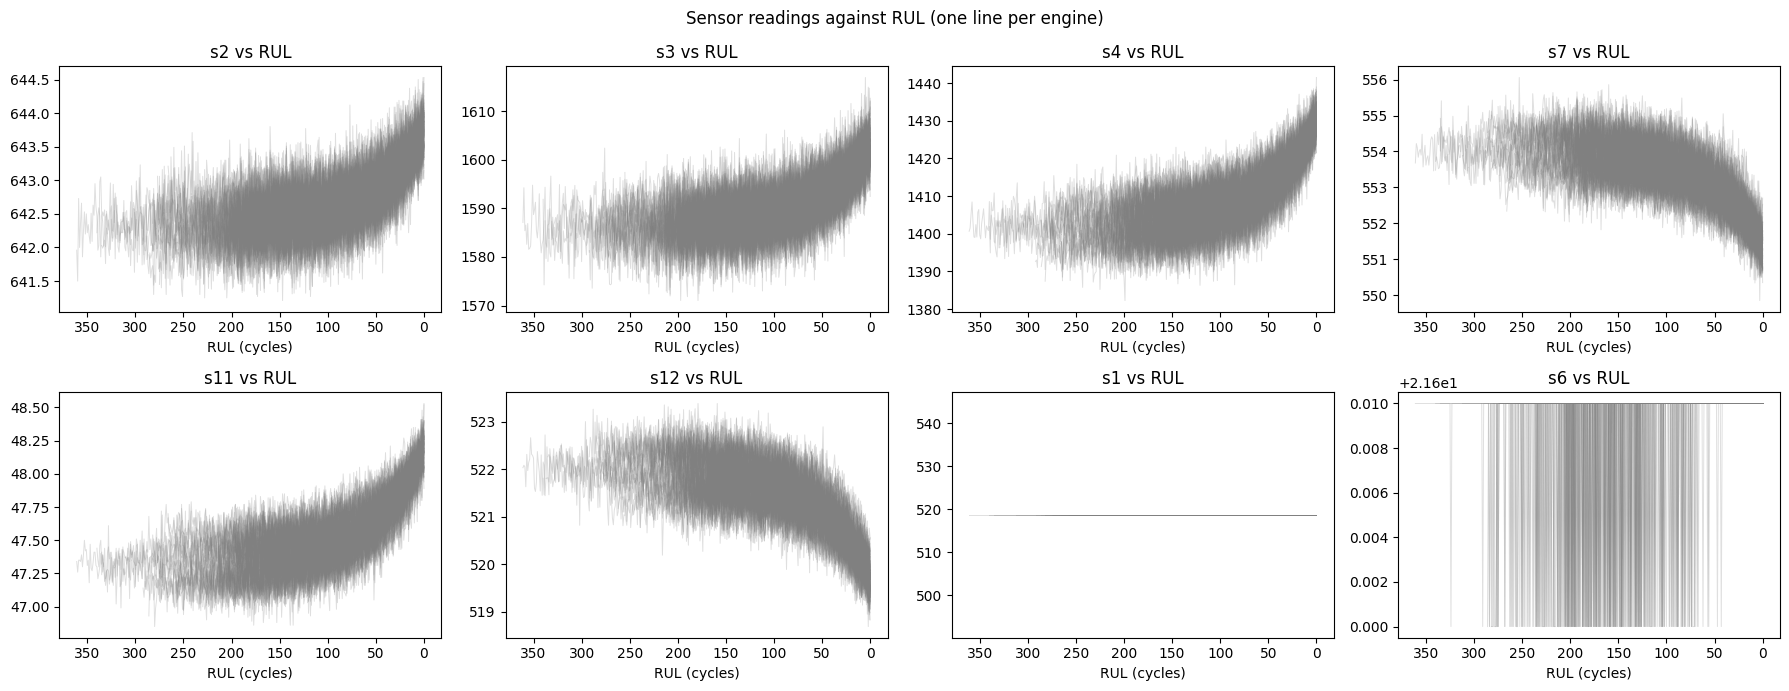
\includegraphics[width=0.9\textwidth]{figures/sensors_vs_rul.png}
\caption{Sensor readings against RUL, one line per training engine.}
\label{fig:sensors}
\end{figure*}

\section{Methodology}
\subsection{Target}
For a training engine with last cycle $T$, the RUL at cycle $t$ is
\begin{equation}
\mathrm{RUL}_t = T - t,
\end{equation}
so the final cycle has $\mathrm{RUL}=0$. The main model uses this uncapped target. The test target is the provided RUL at each engine's last observed cycle.

\subsection{Sensor selection}
We drop any sensor whose standard deviation on the training data is below $0.01$. This removes sensors s1, s5, s6, s10, s16, s18, and s19 and leaves 14 sensors. The rule uses no labels and no test data.

\subsection{Feature engineering}
For each kept sensor $x$ and each engine, at cycle $t$ with window $w=5$ we compute
\begin{align}
\bar{x}_t &= \frac{1}{\min(w,t)}\sum_{k=\max(1,t-w+1)}^{t} x_k, \\
m_t &= \frac{x_t - x_{t-w+1}}{w-1}, \\
h_t &= x_t - \frac{1}{b}\sum_{k=1}^{b} x_k \quad (t \ge b),
\end{align}
the rolling mean, the two-point rolling slope, and the health measure, with baseline length $b=10$. Before enough history exists, the slope is set to zero, and $h_t=0$ for $t<b$ so that early rows never use future cycles. Every feature at cycle $t$ therefore depends only on cycles up to $t$ of the same engine. Together with the cycle number and the 14 raw sensors this yields 57 features.

\subsection{Models}
We compare three models on identical features and folds. The naive baseline predicts the training-fold mean RUL. The Elastic Net minimises squared error with a mixed $\ell_1$ and $\ell_2$ penalty \cite{zou2005en}, with standardised inputs inside a pipeline ($\alpha=1.0$, $\ell_1$ ratio $0.5$). The Random Forest averages decision trees trained on bootstrap samples \cite{breiman2001rf} (200 trees, minimum leaf size 5; scikit-learn's default of all features per split). Hyperparameters were fixed and not tuned.

\subsection{Evaluation protocol}
Rows of the same engine are strongly correlated, so a random row split would leak information between training and validation sets. We therefore use 5-fold \texttt{GroupKFold} on engine ID over the 100 training engines and report the mean and standard deviation across folds. The metrics are
\begin{align}
\mathrm{RMSE} &= \sqrt{\tfrac{1}{n}\textstyle\sum_i (y_i-\hat y_i)^2}, &
\mathrm{MAE} &= \tfrac{1}{n}\textstyle\sum_i |y_i-\hat y_i|,
\end{align}
and MAE is also reported separately for early rows (true RUL $\ge 50$) and late rows (true RUL $<50$). The final models are retrained on all training engines and evaluated once on the test engines at their last cycle.

\section{Results}
\subsection{Window size}
Cross-validated RMSE for rolling windows of 3, 5 and 10 cycles was 34.40, 34.82 and 36.28 (MAE 22.59, 22.85 and 23.76) with a 100-tree Random Forest. Windows 3 and 5 differ by 0.42 RMSE, far below the fold-to-fold standard deviation of about 2, so they are indistinguishable, while 10 is slightly worse. A strict lowest-RMSE rule would pick 3; we kept the pre-set window of 5 for all reported results because the difference is within noise. The sweep reuses the engines used for model comparison, so it is a sanity check and not an independent validation.

\subsection{Cross-validation}
\begin{table}[t]
\centering
\caption{5-fold grouped cross-validation (mean $\pm$ std over folds).}
\label{tab:cv}
\begin{tabular}{lcccc}
\toprule
Model & RMSE & MAE & MAE early & MAE late \\
\midrule
Naive (mean) & 68.87 $\pm$ 1.32 & 56.86 $\pm$ 0.51 & 48.40 $\pm$ 0.71 & 83.31 $\pm$ 0.12 \\
Elastic Net & 40.04 $\pm$ 2.98 & 30.63 $\pm$ 1.56 & 32.96 $\pm$ 2.19 & 23.35 $\pm$ 1.21 \\
Random Forest & 34.78 $\pm$ 1.97 & 22.79 $\pm$ 0.91 & 28.47 $\pm$ 1.11 & 5.04 $\pm$ 0.34 \\
\bottomrule
\end{tabular}
\end{table}

\subsection{Test set}
\begin{table}[t]
\centering
\caption{Test set, 100 engines scored at their last cycle.}
\label{tab:test}
\begin{tabular}{lcccc}
\toprule
Model & RMSE & MAE & MAE early & MAE late \\
\midrule
Naive (mean) & 52.62 & 40.88 & 21.44 & 86.24 \\
Elastic Net & 27.98 & 23.68 & 25.02 & 20.55 \\
Random Forest & 23.34 & 15.58 & 20.54 & 4.02 \\
\bottomrule
\end{tabular}
\end{table}

\subsection{Error analysis}
Fig.~\ref{fig:err} shows out-of-fold predictions for all 20{,}631 training rows. Errors are small close to failure (mean absolute error about 3 cycles for true RUL below 25 and about 7 for 25 to 50) and grow with true RUL: about 22 to 26 cycles from 75 to 200 and well above 100 beyond 275. Predictions for the longest-lived engines level off near 200, so remaining life is underestimated for them. On the test engines the Random Forest has MAE 20.54 for 70 early engines and 4.02 for 30 late engines. The Elastic Net is much worse on late engines (20.55), so the relationship between features and RUL is clearly non-linear. By impurity-based importance the cycle number is the top feature (0.559), followed by the rolling means of s4, s15 and s11 and the health value of s11 (0.088, 0.048, 0.042, 0.038); impurity importances can favour correlated features, so we read them as a rough guide only.

\begin{figure}[t]
\centering
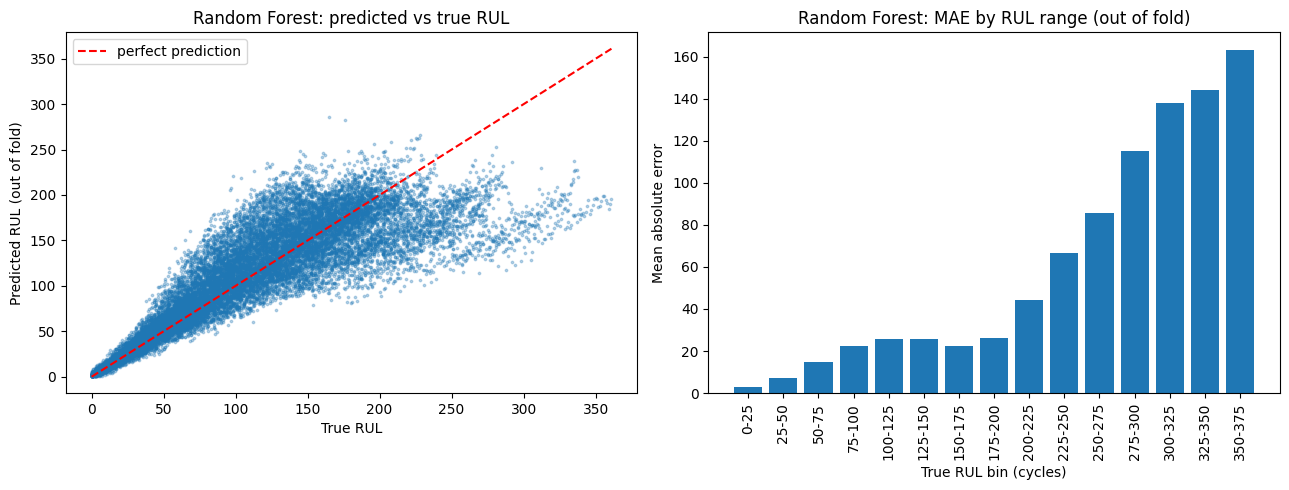
\includegraphics[width=\columnwidth]{figures/error_analysis.png}
\caption{Random Forest, out-of-fold: predicted versus true RUL (left) and mean absolute error by true RUL range (right).}
\label{fig:err}
\end{figure}

\subsection{Capped target}
Many studies cap the training RUL at 125 cycles. The project does not specify a cap, so the main model is uncapped. We trained a capped Random Forest and scored both models against the true, uncapped RUL, since scoring against a capped truth would favour the model trained on that target. With a cap of 125 the Random Forest scored RMSE 46.40 and MAE 28.90 against uncapped RUL, versus 34.78 and 22.79 uncapped. The gap comes from early rows (MAE 36.55 versus 28.47), where a capped model cannot predict above 125; late-stage MAE is almost identical (4.97 versus 5.04). Scoring on uncapped truth favours the uncapped model, as scoring on capped truth would favour the capped one, so we kept the uncapped model because the project's target is the true RUL and it states no cap.

\section{Discussion and Limitations}
The Random Forest beats the naive baseline and the Elastic Net in both cross-validation and test, and its advantage is largest near failure, where it is more than four times more accurate than the Elastic Net. Test errors (RMSE 23.34) are lower than cross-validation errors (34.78), but the two are not directly comparable: cross-validation scores every row of held-out engines across their whole lifetime, including early cycles with RUL up to 361, whereas the test score uses one cycle per engine at its cutoff. The naive baseline shows the same shift (early-stage MAE 48.40 in cross-validation versus 21.44 on test), which suggests the test targets are less extreme. The cycle number is the most important feature, so the model partly relies on engine age, which varies widely between engines (128 to 362 cycles). We note the following limitations. Model settings were fixed, not tuned. The window size was chosen by cross-validation on the same engines used for model comparison, so cross-validation scores are slightly optimistic. The baseline length and the early/late threshold were set by hand. The test score uses one cycle per engine over 100 engines and is therefore noisy, and cross-validation and test scores measure different things, so their closeness is not evidence against overfitting. Only FD001, with one operating condition, is used. Finally, fixed rolling windows may miss long degradation trajectories whose timing differs between engines.

\section{Conclusion and Future Work}
A Random Forest on engineered rolling features predicts RUL on FD001 with a test MAE of 15.58 cycles and a cross-validated MAE of 22.79, clearly better than a naive baseline and a linear Elastic Net, and it is accurate close to failure (test MAE 4.02) but much less so early in life. The next phase trains a sequence model on fixed-length raw sensor windows, using the same engine-level split and metrics, and examines whether combining it with the engineered features is beneficial.

\begin{thebibliography}{10}
\bibitem{saxena2008damage} A.~Saxena, K.~Goebel, D.~Simon, and N.~Eklund, ``Damage propagation modeling for aircraft engine run-to-failure simulation,'' in \emph{Proc.\ Int.\ Conf.\ Prognostics and Health Management}, 2008.
\bibitem{saxena2008cmapss} A.~Saxena and K.~Goebel, ``Turbofan engine degradation simulation data set,'' NASA Prognostics Data Repository, 2008.
\bibitem{hochreiter1997lstm} S.~Hochreiter and J.~Schmidhuber, ``Long short-term memory,'' \emph{Neural Computation}, vol.~9, no.~8, pp.~1735--1780, 1997.
\bibitem{breiman2001rf} L.~Breiman, ``Random forests,'' \emph{Machine Learning}, vol.~45, no.~1, pp.~5--32, 2001.
\bibitem{zou2005en} H.~Zou and T.~Hastie, ``Regularization and variable selection via the elastic net,'' \emph{J.\ Royal Statistical Society B}, vol.~67, no.~2, pp.~301--320, 2005.
\bibitem{heimes2008rnn} F.~O.~Heimes, ``Recurrent neural networks for remaining useful life estimation,'' in \emph{Proc.\ Int.\ Conf.\ Prognostics and Health Management}, 2008.
\bibitem{babu2016cnn} G.~S.~Babu, P.~Zhao, and X.-L.~Li, ``Deep convolutional neural network based regression approach for estimation of remaining useful life,'' in \emph{Database Systems for Advanced Applications (DASFAA)}, 2016, pp.~214--228.
\bibitem{pedregosa2011sklearn} F.~Pedregosa \emph{et al.}, ``Scikit-learn: Machine learning in Python,'' \emph{J.\ Machine Learning Research}, vol.~12, pp.~2825--2830, 2011.
\end{thebibliography}

\end{document}
